\section{问题二：极端风速下的配重调节}

\subsection{原参数在风速 $36\,\mathrm{m/s}$ 下的系统状态}

问题二仅将海面风速提高至 $36\,\mathrm{m/s}$，其余布放条件、构件参数及模型假设均与问题一保持一致。因此，本问不重新建立新的受力模型，而直接沿用问题一中浮标、四节钢管、钢桶--重物球以及锚链的静力平衡关系，并继续以浮标吃水深度 $\delta$ 为搜索变量。对给定的重物球质量 $m_{\mathrm s}$，按照问题一的计算流程得到模型水深 $H(\delta)$，再利用二分法求解
\begin{equation}
  H(\delta)=18.
  \label{eq:q2-depth-closure}
\end{equation}
求得平衡状态后，按照第 4 节符号说明中的统一记号，记录四节钢管倾角 $\theta_i$、钢桶倾角 $\theta_{\mathrm d}$、锚端夹角 $\varphi_{\mathrm a}$、浮标吃水深度 $\delta$ 以及游动半径 $r$。

首先保持问题一所用重物球质量 $m_{\mathrm s}=1200\,\mathrm{kg}$ 不变。将 $v_{\mathrm w}=36\,\mathrm{m/s}$ 代入问题一模型，求得各项结果如表\ref{tab:q2-original}所示。

\begin{table}[H]
  \centering
  \caption{风速 $36\,\mathrm{m/s}$、重物球质量 $1200\,\mathrm{kg}$ 时的系统状态}
  \label{tab:q2-original}
  \begin{tabular}{lc}
    \toprule
    指标 & 计算结果 \\
    \midrule
    第1节钢管倾角 $\theta_1$ & $9.1509^{\circ}$ \\
    第2节钢管倾角 $\theta_2$ & $9.2059^{\circ}$ \\
    第3节钢管倾角 $\theta_3$ & $9.2616^{\circ}$ \\
    第4节钢管倾角 $\theta_4$ & $9.3180^{\circ}$ \\
    钢桶倾角 $\theta_{\mathrm d}$ & $9.4458^{\circ}$ \\
    锚端夹角 $\varphi_{\mathrm a}$ & $20.8874^{\circ}$ \\
    浮标吃水深度 $\delta$ & $0.7198\,\mathrm{m}$ \\
    浮标游动半径 $r$ & $18.8720\,\mathrm{m}$ \\
    \bottomrule
  \end{tabular}
\end{table}

由表\ref{tab:q2-original}可见，原 $1200\,\mathrm{kg}$ 配重下，钢桶倾角为 $9.4458^{\circ}$，超过题目给出的 $5^{\circ}$ 限制；同时锚端锚链切线与海床夹角为 $20.8874^{\circ}$，也超过 $16^{\circ}$ 的安全上限。因此，问题一中的原配重方案不能直接用于 $36\,\mathrm{m/s}$ 风速工况，需要增加重物球质量。

在该工况下，锚链处于完全悬起状态，卧底长度为零。锚链形状仍按问题一的处理方式，将 II 型锚链按单节链环长度离散，并由各链环两端张力的受力平衡和链环自身的力矩平衡逐节递推得到。

\subsection{重物球质量的调节}

保持 II 型锚链和 $22.05\,\mathrm{m}$ 锚链总长不变，将重物球质量 $m_{\mathrm s}$ 作为本问唯一调节变量。对于每一个给定的 $m_{\mathrm s}$，均按照问题一完全相同的顺序求解：先由浮标受力确定顶部张力，再逐节计算四节钢管和钢桶姿态；重物球的水中有效重力通过钢桶下端连接点传递给锚链；随后对锚链各链环继续进行受力和力矩平衡递推，最后通过式\eqref{eq:q2-depth-closure}求解吃水深度 $\delta$。

为使系统同时满足水声通信设备和锚泊安全要求，建立如下单变量约束模型：
\begin{equation}
  \min m_{\mathrm s},
  \label{eq:q2-objective}
\end{equation}
\begin{equation}
  \text{s.t.}\quad
  \begin{cases}
    H(\delta;m_{\mathrm s})=18,\\
    \theta_{\mathrm d}(m_{\mathrm s})\leq 5^{\circ},\\
    \varphi_{\mathrm a}(m_{\mathrm s})\leq 16^{\circ},\\
    0<\delta<2.
  \end{cases}
  \label{eq:q2-constraints}
\end{equation}

数值求解时，先从 $1200\,\mathrm{kg}$ 起按 $10\,\mathrm{kg}$ 步长增加重物球质量。每取一个质量，内层均继续使用问题一的二分法重新求解 $H(\delta)=18$，并判断 $\theta_{\mathrm d}$ 与 $\varphi_{\mathrm a}$ 是否同时满足约束。得到可行区间后，再对重物球质量进行二分搜索，以确定临界质量。

质量搜索结果表明，在理论临界状态下钢桶倾角已经低于 $5^{\circ}$，而锚端夹角恰好达到 $16^{\circ}$，因此本问实际起控制作用的是锚端夹角约束。由 $\varphi_{\mathrm a}=16^{\circ}$ 得到理论临界质量
\begin{equation}
  m_{\mathrm s}^{\min}=2219.45\,\mathrm{kg}.
  \label{eq:q2-critical-mass}
\end{equation}
若按 $10\,\mathrm{kg}$ 为质量调整步长，则最小可行整数方案为 $2220\,\mathrm{kg}$。此时
\[
  \theta_{\mathrm d}=4.5119^{\circ},\qquad
  \varphi_{\mathrm a}=15.9969^{\circ},
\]
虽然已经满足题目约束，但锚端夹角与 $16^{\circ}$ 上限非常接近。为避免数值舍入和实际参数微小波动使方案重新越过约束边界，本文在不改变问题一模型的前提下，将最终配重取为
\begin{equation}
  \boxed{m_{\mathrm s}=2250\,\mathrm{kg}}.
  \label{eq:q2-selected-mass}
\end{equation}

重物球质量对两项角度指标的影响如图\ref{fig:q2-mass-constraints}所示。随着配重增加，钢桶倾角和锚端夹角均单调减小；其中锚端夹角首先达到约束边界，验证了其为本问的控制约束。
\begin{figure}[H]
  \centering
  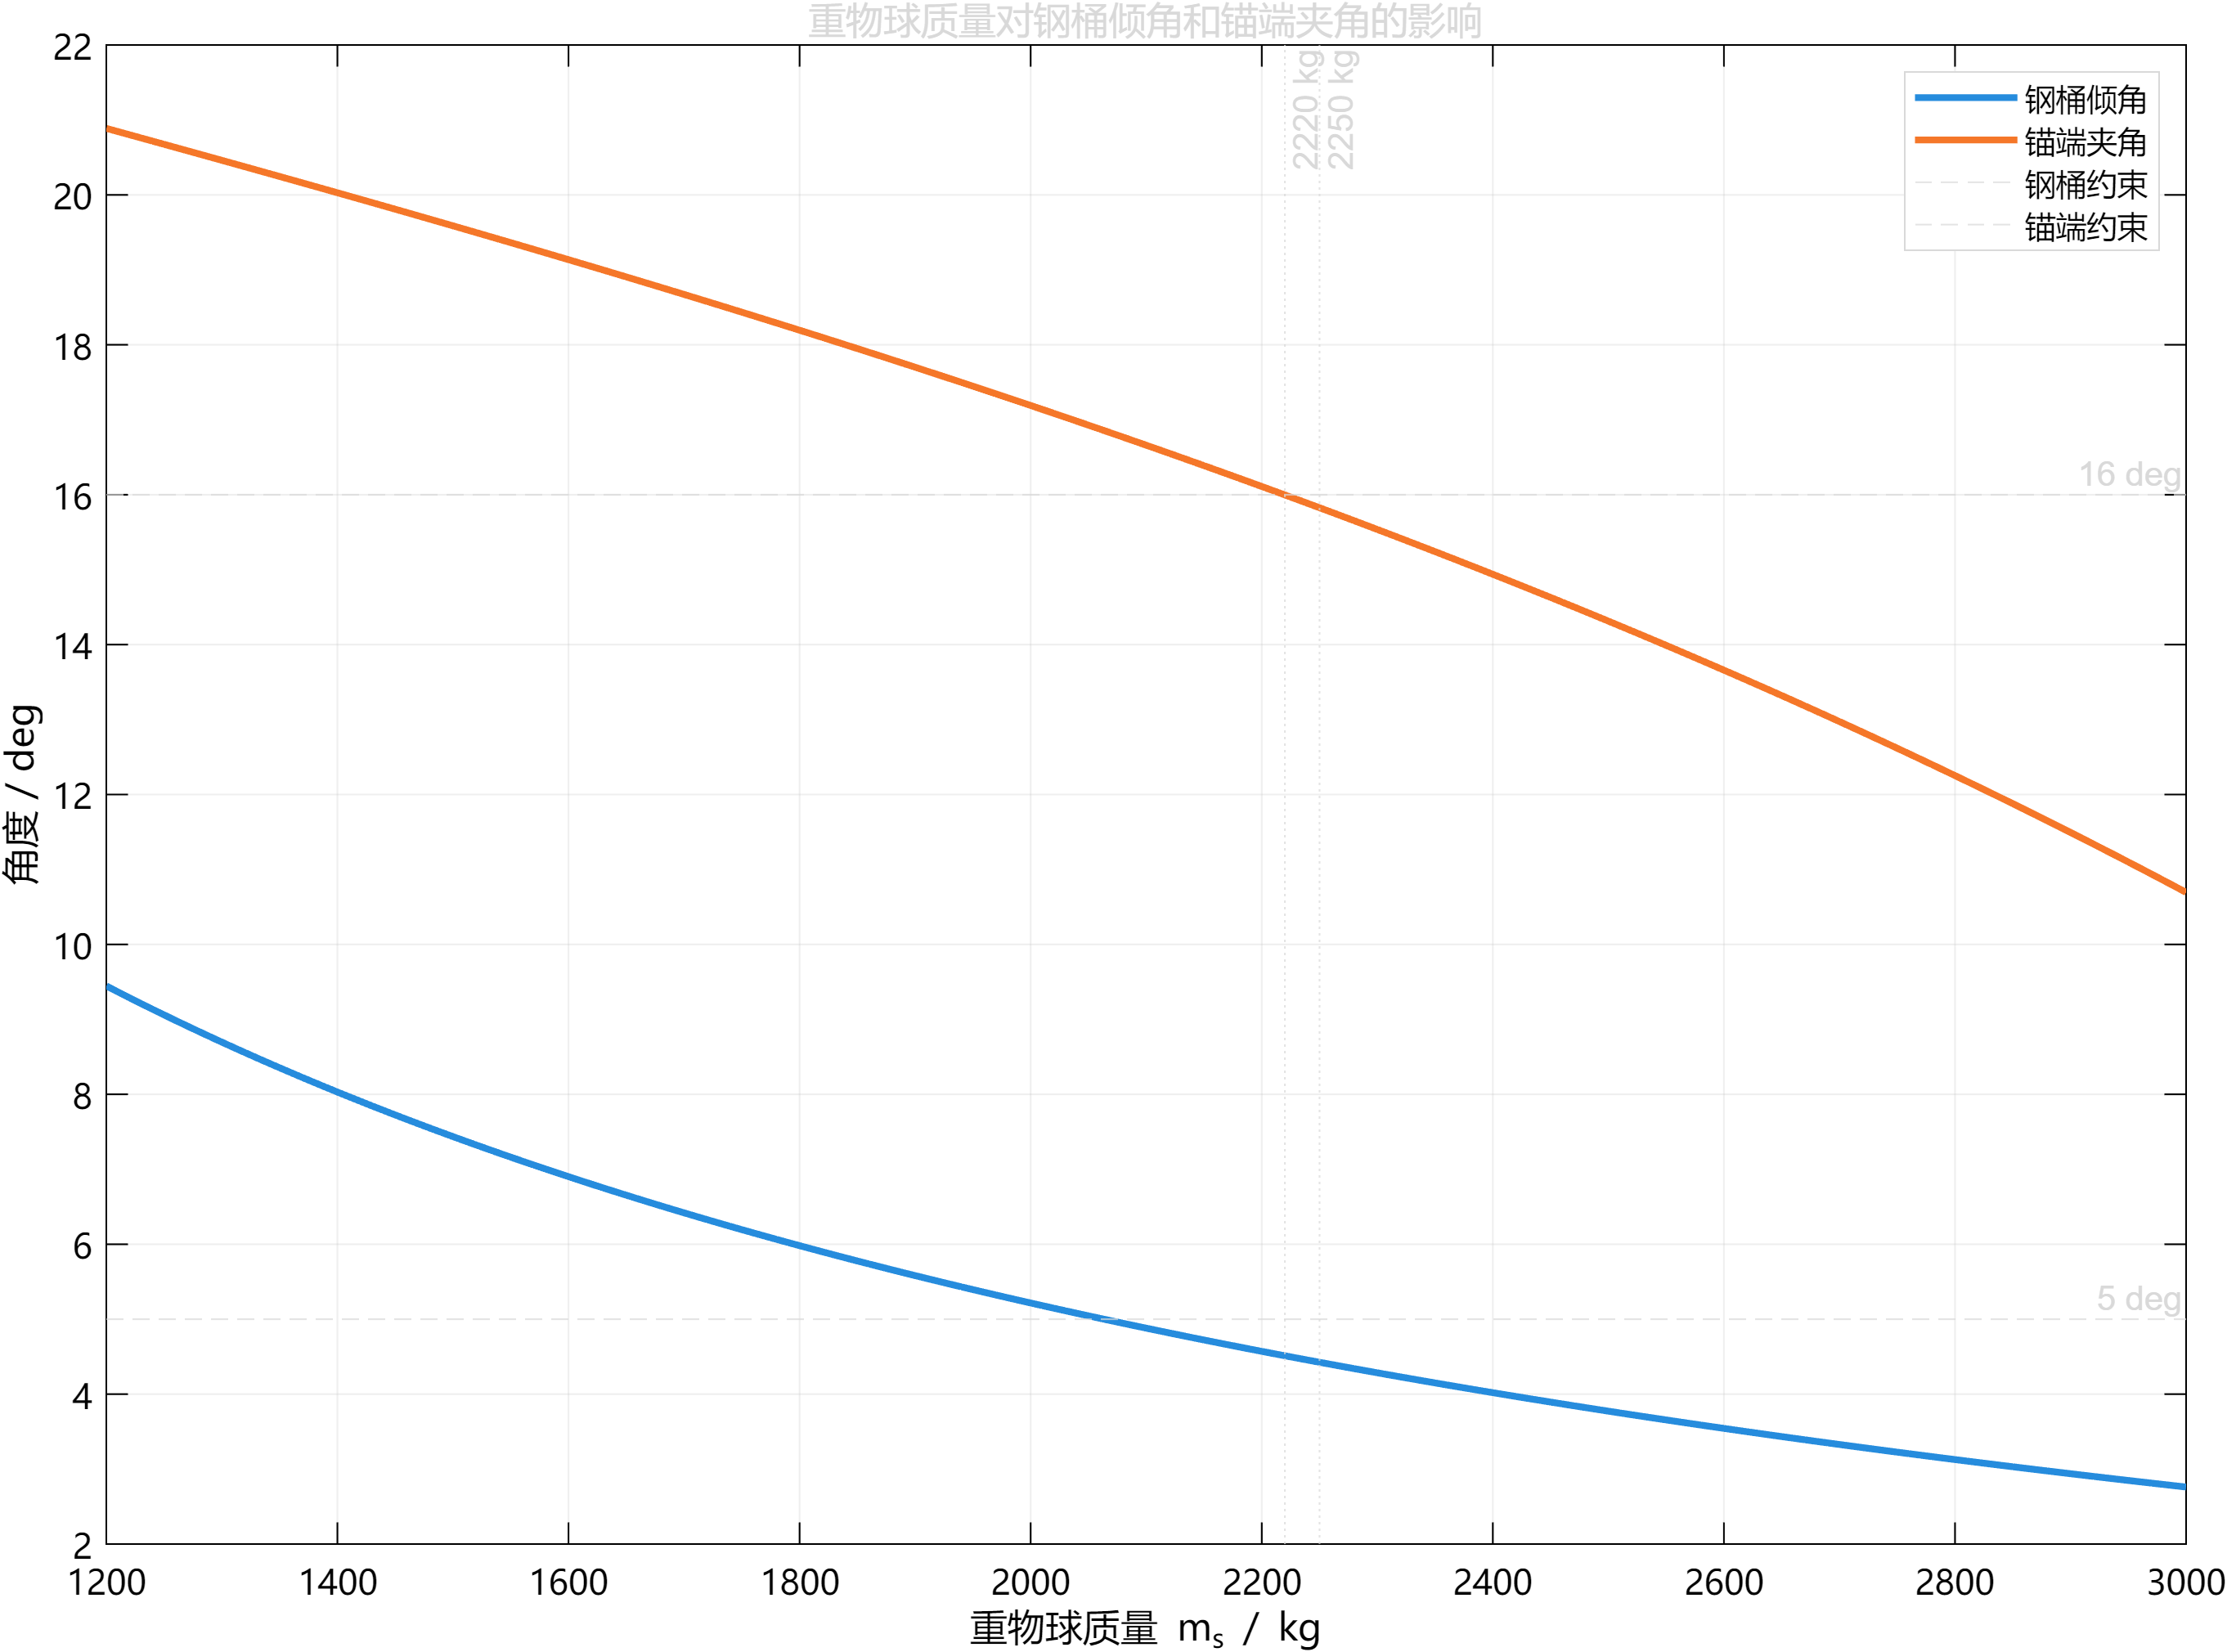
\includegraphics[width=0.88\linewidth]{figures/q2_mass_constraints.png}
  \caption{重物球质量对钢桶倾角和锚端夹角的影响}
  \label{fig:q2-mass-constraints}
\end{figure}

\subsection{调节后的系统状态}

将 $m_{\mathrm s}=2250\,\mathrm{kg}$ 代回问题一模型，并再次求解 $H(\delta)=18$，得到调节后的系统状态如表\ref{tab:q2-adjusted}所示。

\begin{table}[H]
  \centering
  \caption{风速 $36\,\mathrm{m/s}$、重物球质量 $2250\,\mathrm{kg}$ 时的系统状态}
  \label{tab:q2-adjusted}
  \begin{tabular}{lc}
    \toprule
    指标 & 计算结果 \\
    \midrule
    第1节钢管倾角 $\theta_1$ & $4.3413^{\circ}$ \\
    第2节钢管倾角 $\theta_2$ & $4.3571^{\circ}$ \\
    第3节钢管倾角 $\theta_3$ & $4.3730^{\circ}$ \\
    第4节钢管倾角 $\theta_4$ & $4.3890^{\circ}$ \\
    钢桶倾角 $\theta_{\mathrm d}$ & $4.4251^{\circ}$ \\
    锚端夹角 $\varphi_{\mathrm a}$ & $15.8260^{\circ}$ \\
    浮标吃水深度 $\delta$ & $0.9928\,\mathrm{m}$ \\
    浮标游动半径 $r$ & $18.5315\,\mathrm{m}$ \\
    \bottomrule
  \end{tabular}
\end{table}

调节前后锚链的空间形态对比如图\ref{fig:q2-chain-shapes}所示。两种配重下锚链均为全长悬起状态；增加配重后，锚链的水平展距减小，与表中浮标游动半径的变化一致。
\begin{figure}[H]
  \centering
  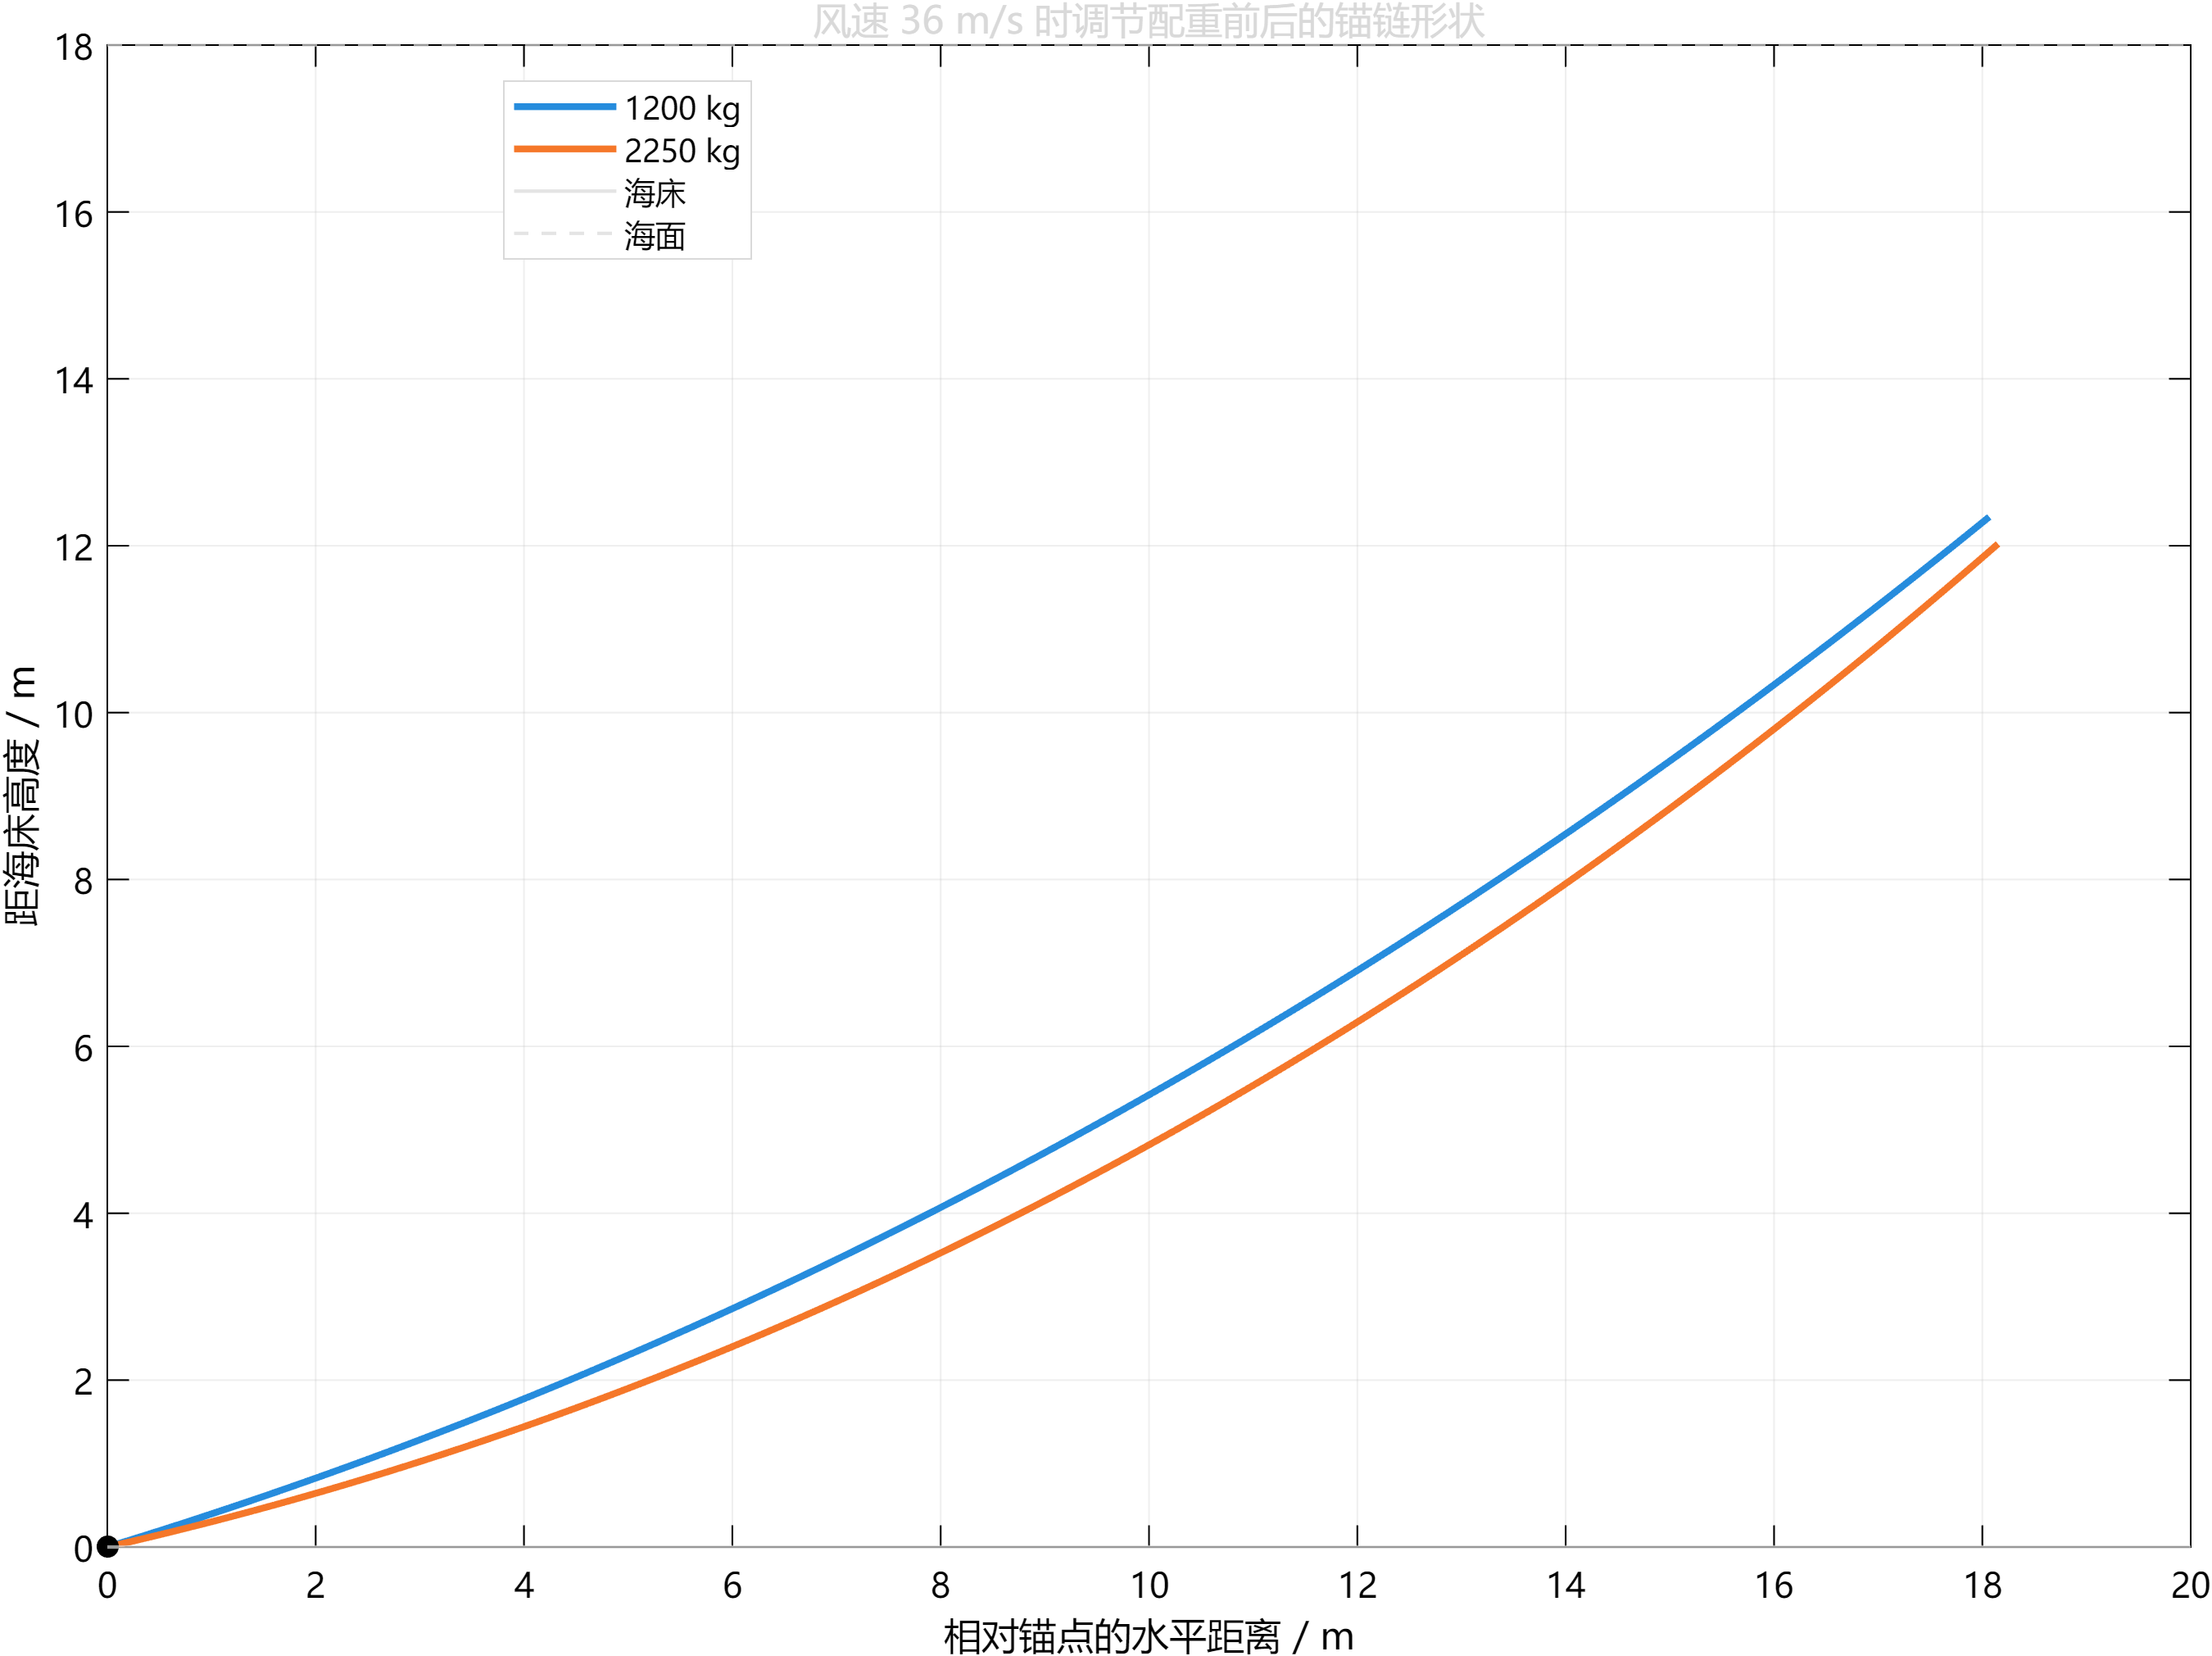
\includegraphics[width=0.88\linewidth]{figures/q2_chain_shapes.png}
  \caption{风速 $36\,\mathrm{m/s}$ 时调节配重前后的锚链形状}
  \label{fig:q2-chain-shapes}
\end{figure}

调节后钢桶倾角由 $9.4458^{\circ}$ 降至 $4.4251^{\circ}$，满足不超过 $5^{\circ}$ 的要求；锚端夹角由 $20.8874^{\circ}$ 降至 $15.8260^{\circ}$，满足不超过 $16^{\circ}$ 的要求。与此同时，浮标游动半径由 $18.8720\,\mathrm{m}$ 略减至 $18.5315\,\mathrm{m}$，而吃水深度由 $0.7198\,\mathrm{m}$ 增至 $0.9928\,\mathrm{m}$。这说明增加重物球质量能够明显减小钢桶和钢管的倾斜程度，并降低锚端夹角，但会使浮标承担更大的竖向系泊载荷，从而增加吃水深度。

因此，在问题一模型、II 型锚链 $22.05\,\mathrm{m}$ 及水深 $18\,\mathrm{m}$ 的条件下，风速提高到 $36\,\mathrm{m/s}$ 后原 $1200\,\mathrm{kg}$ 配重不满足约束；理论临界质量约为 $2219.45\,\mathrm{kg}$，按 $10\,\mathrm{kg}$ 步长最小可行质量为 $2220\,\mathrm{kg}$。考虑到锚端夹角在临界方案下几乎贴近 $16^{\circ}$ 上限，最终采用 $2250\,\mathrm{kg}$ 作为问题二的配重方案。
